% Options for packages loaded elsewhere
\PassOptionsToPackage{unicode}{hyperref}
\PassOptionsToPackage{hyphens}{url}
\PassOptionsToPackage{dvipsnames,svgnames*,x11names*}{xcolor}
%
\documentclass[
]{krantz}
\usepackage{amsmath,amssymb}
\usepackage{lmodern}
\usepackage{ifxetex,ifluatex}
\ifnum 0\ifxetex 1\fi\ifluatex 1\fi=0 % if pdftex
  \usepackage[T1]{fontenc}
  \usepackage[utf8]{inputenc}
  \usepackage{textcomp} % provide euro and other symbols
\else % if luatex or xetex
  \usepackage{unicode-math}
  \defaultfontfeatures{Scale=MatchLowercase}
  \defaultfontfeatures[\rmfamily]{Ligatures=TeX,Scale=1}
\fi
% Use upquote if available, for straight quotes in verbatim environments
\IfFileExists{upquote.sty}{\usepackage{upquote}}{}
\IfFileExists{microtype.sty}{% use microtype if available
  \usepackage[]{microtype}
  \UseMicrotypeSet[protrusion]{basicmath} % disable protrusion for tt fonts
}{}
\makeatletter
\@ifundefined{KOMAClassName}{% if non-KOMA class
  \IfFileExists{parskip.sty}{%
    \usepackage{parskip}
  }{% else
    \setlength{\parindent}{0pt}
    \setlength{\parskip}{6pt plus 2pt minus 1pt}}
}{% if KOMA class
  \KOMAoptions{parskip=half}}
\makeatother
\usepackage{xcolor}
\IfFileExists{xurl.sty}{\usepackage{xurl}}{} % add URL line breaks if available
\IfFileExists{bookmark.sty}{\usepackage{bookmark}}{\usepackage{hyperref}}
\hypersetup{
  pdftitle={Exploring Modeling with Data and Differential Equations Using R},
  pdfauthor={John M. Zobitz},
  colorlinks=true,
  linkcolor=Maroon,
  filecolor=Maroon,
  citecolor=Blue,
  urlcolor=Blue,
  pdfcreator={LaTeX via pandoc}}
\urlstyle{same} % disable monospaced font for URLs
\usepackage{longtable,booktabs,array}
\usepackage{calc} % for calculating minipage widths
% Correct order of tables after \paragraph or \subparagraph
\usepackage{etoolbox}
\makeatletter
\patchcmd\longtable{\par}{\if@noskipsec\mbox{}\fi\par}{}{}
\makeatother
% Allow footnotes in longtable head/foot
\IfFileExists{footnotehyper.sty}{\usepackage{footnotehyper}}{\usepackage{footnote}}
\makesavenoteenv{longtable}
\usepackage{graphicx}
\makeatletter
\def\maxwidth{\ifdim\Gin@nat@width>\linewidth\linewidth\else\Gin@nat@width\fi}
\def\maxheight{\ifdim\Gin@nat@height>\textheight\textheight\else\Gin@nat@height\fi}
\makeatother
% Scale images if necessary, so that they will not overflow the page
% margins by default, and it is still possible to overwrite the defaults
% using explicit options in \includegraphics[width, height, ...]{}
\setkeys{Gin}{width=\maxwidth,height=\maxheight,keepaspectratio}
% Set default figure placement to htbp
\makeatletter
\def\fps@figure{htbp}
\makeatother
\setlength{\emergencystretch}{3em} % prevent overfull lines
\providecommand{\tightlist}{%
  \setlength{\itemsep}{0pt}\setlength{\parskip}{0pt}}
\setcounter{secnumdepth}{5}
\usepackage{tikz}
\usepackage{pgfplots}
\usepackage{amsmath}
\usetikzlibrary{calc}
\usetikzlibrary{arrows,matrix,positioning}
\usepackage{float}
\floatplacement{figure}{H}
\usepackage[shortlabels]{enumitem}
\usepackage{mathtools}
\pgfplotsset{compat=1.17}



\usepackage{booktabs}
\usepackage{longtable}
\usepackage[bf,singlelinecheck=off]{caption}
\captionsetup[table]{labelsep=space}
\captionsetup[figure]{labelsep=space}
\usepackage[scale=.8]{sourcecodepro}

\usepackage{framed,color}
\definecolor{shadecolor}{RGB}{248,248,248}

\renewcommand{\textfraction}{0.05}
\renewcommand{\topfraction}{0.8}
\renewcommand{\bottomfraction}{0.8}
\renewcommand{\floatpagefraction}{0.75}

\renewenvironment{quote}{\begin{VF}}{\end{VF}}
\let\oldhref\href
\renewcommand{\href}[2]{#2\footnote{\url{#1}}}

\makeatletter
\newenvironment{kframe}{%
\medskip{}
\setlength{\fboxsep}{.8em}
 \def\at@end@of@kframe{}%
 \ifinner\ifhmode%
  \def\at@end@of@kframe{\end{minipage}}%
  \begin{minipage}{\columnwidth}%
 \fi\fi%
 \def\FrameCommand##1{\hskip\@totalleftmargin \hskip-\fboxsep
 \colorbox{shadecolor}{##1}\hskip-\fboxsep
     % There is no \\@totalrightmargin, so:
     \hskip-\linewidth \hskip-\@totalleftmargin \hskip\columnwidth}%
 \MakeFramed {\advance\hsize-\width
   \@totalleftmargin\z@ \linewidth\hsize
   \@setminipage}}%
 {\par\unskip\endMakeFramed%
 \at@end@of@kframe}
\makeatother

%\renewenvironment{Shaded}{\begin{kframe}}{\end{kframe}}
\usepackage{url}
\usepackage{makeidx}
\makeindex

\urlstyle{tt}

\usepackage{amsthm}
\makeatletter
\def\thm@space@setup{%
  \thm@preskip=8pt plus 2pt minus 4pt
  \thm@postskip=\thm@preskip
}
\makeatother

\frontmatter
\usepackage{booktabs}
\usepackage{longtable}
\usepackage{array}
\usepackage{multirow}
\usepackage{wrapfig}
\usepackage{float}
\usepackage{colortbl}
\usepackage{pdflscape}
\usepackage{tabu}
\usepackage{threeparttable}
\usepackage{threeparttablex}
\usepackage[normalem]{ulem}
\usepackage{makecell}
\usepackage{xcolor}
\ifluatex
  \usepackage{selnolig}  % disable illegal ligatures
\fi
\newlength{\cslhangindent}
\setlength{\cslhangindent}{1.5em}
\newlength{\csllabelwidth}
\setlength{\csllabelwidth}{3em}
\newenvironment{CSLReferences}[2] % #1 hanging-ident, #2 entry spacing
 {% don't indent paragraphs
  \setlength{\parindent}{0pt}
  % turn on hanging indent if param 1 is 1
  \ifodd #1 \everypar{\setlength{\hangindent}{\cslhangindent}}\ignorespaces\fi
  % set entry spacing
  \ifnum #2 > 0
  \setlength{\parskip}{#2\baselineskip}
  \fi
 }%
 {}
\usepackage{calc}
\newcommand{\CSLBlock}[1]{#1\hfill\break}
\newcommand{\CSLLeftMargin}[1]{\parbox[t]{\csllabelwidth}{#1}}
\newcommand{\CSLRightInline}[1]{\parbox[t]{\linewidth - \csllabelwidth}{#1}\break}
\newcommand{\CSLIndent}[1]{\hspace{\cslhangindent}#1}

\title{Exploring Modeling with Data and Differential Equations Using R}
\author{John M. Zobitz}
\date{Version 2.0.0}

\usepackage{amsthm}
\newtheorem{theorem}{Theorem}[chapter]
\newtheorem{lemma}{Lemma}[chapter]
\newtheorem{corollary}{Corollary}[chapter]
\newtheorem{proposition}{Proposition}[chapter]
\newtheorem{conjecture}{Conjecture}[chapter]
\theoremstyle{definition}
\newtheorem{definition}{Definition}[chapter]
\theoremstyle{definition}
\newtheorem{example}{Example}[chapter]
\theoremstyle{definition}
\newtheorem{exercise}{Exercise}[chapter]
\theoremstyle{definition}
\newtheorem{hypothesis}{Hypothesis}[chapter]
\theoremstyle{remark}
\newtheorem*{remark}{Remark}
\newtheorem*{solution}{Solution}
\begin{document}
\maketitle

% you may need to leave a few empty pages before the dedication page

%\cleardoublepage\newpage\thispagestyle{empty}\null
%\cleardoublepage\newpage\thispagestyle{empty}\null
%\cleardoublepage\newpage
\thispagestyle{empty}

\begin{center}
To my parents Joan and Francis,

who gave me strong roots from which to grow.

To my wife Shannon,

who provides me the support to keep my trunk from breaking.

To my children Colin, Grant, Phoebe,

who are the branches that support the emerald green leaves.

Kiitos. Amor a todos.
%\includegraphics{images/dedication.pdf}
\end{center}

\setlength{\abovedisplayskip}{-5pt}
\setlength{\abovedisplayshortskip}{-5pt}

{
\hypersetup{linkcolor=}
\setcounter{tocdepth}{1}
\tableofcontents
}
\listoftables
\listoffigures
\hypertarget{welcome}{%
\chapter*{Welcome}\label{welcome}}


This book is written for you: the student learning about modeling and differential equations. Perhaps you first encountered models, differential equations, and better yet, building plausible models from data in your Calculus course.

This book sits ``at the intersection'' of several different mathematics courses: differential equations, linear algebra, statistics, calculus, data science - as well as the partner disciplines of biology, chemsitry, physics, business, and economics. An important idea is one of \emph{transference} where a differential equation model applied in once context can also be applied (perhaps with different variable names) in a separate context.

I intentionally emphasize models from biology and the environmental sciences, but throughout the text you can find examples from the other disciplines. I hope you see the connections of this content to your own intended major.

This book is divided into 4 parts:

\begin{enumerate}
\def\labelenumi{\arabic{enumi}.}
\tightlist
\item
  Models with differential equations
\item
  Parameterizing models with data
\item
  Stability analysis for differential equations.
\item
  Stochastic differential equations
\end{enumerate}

You may notice the interwoven structure for this book: models are introduced first, followed by data analysis and parameter estimation, returning back to analyzing models, and ending with simulating random (stochastic) models.

Unsure what about all these topics mean? Do not worry! The topics are presented with a ``modeling first'' paradigm that first introduces models, and equally important, how data are used to inform a model. This ``conversation'' between models and data are important to help build plausibility and confidence in a model. Stability analysis helps to solidify the connection between models and parameters (which may change the underlying dynamical stability). Finally the notion of \emph{randomness} is extended with the introduction of stochastic differential equations.

Unifying all of these approaches is the idea of developing workflows for analysis, visualization results, and interpreting any results in the context of the problem.

\hypertarget{computational-code}{%
\section*{Computational code}\label{computational-code}}


This book makes heavy use of the \texttt{R} programming language, and unabashedly develops programming principles using the \texttt{tidyverse} syntax and programming approach. This is intentional to facilitate direct connections to courses in introductory data science or data visualization. Throughout my years learning (and teaching) different programming languages I have found \texttt{R} to be the most versatile and adaptable. The \texttt{tidyverse} syntax, in my opinion, is transformed my own thinking about sustainable computation and modeling processes - and I hope it does for you as well.

There is a companion \texttt{R} package available called \texttt{demodelr} to run programs and functions in the text. Instructions to install this package are given in Section \ref{r-intro-02}. The minimum version of R Version 4.0.2 (2020-06-22) (\protect\hyperlink{ref-R-base}{R Core Team 2021}) and RStudio is Version 1.4.1717 (\protect\hyperlink{ref-rstudio_team_rstudio_2020}{RStudio Team 2020})

The \texttt{demodelr} package uses the following \texttt{R} packages:

\begin{itemize}
\tightlist
\item
  \texttt{tidyverse} (and the associated packages) (Version 1.3.1) (\protect\hyperlink{ref-tidyverse2019}{Wickham et al. 2019})
\item
  \texttt{GGally} (Version 2.1.2) (\protect\hyperlink{ref-R-GGally}{Schloerke et al. 2021})
\item
  \texttt{formula.tools} (Version 1.7.1) (\protect\hyperlink{ref-R-formula.tools}{Brown 2018})
\item
  \texttt{expm} (Version 0.999-6) (\protect\hyperlink{ref-R-expm}{Goulet et al. 2021})
\end{itemize}

\hypertarget{questions-comments-issues}{%
\section*{Questions? Comments? Issues?}\label{questions-comments-issues}}


Feel free to file an issue with the \texttt{demodelr} package to my \href{https://github.com/jmzobitz/ModelingWithR/issues}{github}

\hypertarget{about-the-cover}{%
\section*{About the cover}\label{about-the-cover}}


The cover art was taken by Shannon Zobitz during a hike at \href{https://visitleppavirta.fi/en/service/orinoro-gorge}{Orinoro Gorge} in Finland. The photo is indicative of several things: (1) the journey ahead as you commence learning about modeling, differential equations, and \texttt{R}, (2) the occasional roots in the path that may cause you to stumble (such as coding errors). Everyone makes them, so you are in good company. (3) the yellow markings on the trees indicate the way forward. May this textbook be the guide for you as you progress over the hill and onward. Let's get started!

\hypertarget{acknowledgments}{%
\section*{Acknowledgments}\label{acknowledgments}}


This book has been developed over the course of several years in a variety of places: two continents, between meetings, in the early mornings, at coffee shops, or while waiting for practices to end. Special thanks are to the following:

\begin{itemize}
\item
  \textbf{Augsburg University:} You have been my professional home for over a decade and given me the space and support to be intellectually creative in my teaching and scholarship. Special thanks to my Mathematics, Statistics, and Computer Science Department colleagues - it is a joy to work with all of you.
\item
  \textbf{Augsburg University students:} Thank you for your interest and engagement in this topic, allowing me to test ideas in an upper division course titled (wait for it \ldots) \emph{Modeling and Differential Equations in the Biological and Natural Sciences}. While the course title is a mouthful, you provided concise, honest, and insightful feedback, shaping this text. I am forever indebted to you.
\item
  \textbf{My family:} Shannon, Colin, Grant, and Phoebe for humoring me (and my occasional grumpiness) while this project has been completed.
\end{itemize}

\mainmatter

\hypertarget{modeling-rates-03}{%
\chapter{Modeling With Rates of Change}\label{modeling-rates-03}}

Section \ref{intro-01} provided examples for modeling with rates of change, and Section \ref{r-intro-02} introduced the computational and visualization software \texttt{R} and \texttt{RStudio}. how we can translate equations with rates of change to understand phenomena. The focus for this section will be on taking a contextual description and starting to develop differential equation models for them.

Oftentimes when we construct differential equations from a contextual description we bring our own understanding and knowledge to this situation. How \emph{you} may write down the differential equation may be different from someone else - \emph{do not worry!} This is the fun part of modeling: models can be considered testable hypotheses that can be refined when confronted with data. Let's get started

\hypertarget{competing-plant-species-and-equilibrium-solutions}{%
\section{Competing plant species and equilibrium solutions}\label{competing-plant-species-and-equilibrium-solutions}}

Consider the following context to develop a mathematical model:

\begin{quote}
A newly introduced plant species is introduced to a region. It competes with another established species for nutrients (and is a better competitor). However, the growth rate of the new species is proportional to the difference between the current number of established species and the number of new species. You may assume that the number of established species is a constant \emph{E}.
\end{quote}

For this problem we will start by naming our variables. Let \(N\) represent number of new species and \(E\) the number of established species. We will break this down accordingly:

\begin{itemize}
\tightlist
\item
  \emph{``the growth rate of the new species''} describes the rate of change, or derivative, expressed as \(\displaystyle \frac{dN}{dt}\).
\item
  \emph{``is proportional to the difference between the current number of established species and the number of new species''} means \(\displaystyle \alpha \cdot (E-N)\), where \(\alpha\) is the proportionality constant. Including this parameter helps to avoid assuming we have a 1:1 correspondence between the growth rate of the new species and the population difference.
\item
  \emph{``and is a better competitor''} helps to explain why the term is \(\displaystyle \alpha \cdot (E-N)\) instead of \(\displaystyle \alpha \cdot (N-E)\). We know that the newly established species will start out in much smaller numbers than \(N\). But since it is a better competitor, we would expect its rate to increase initially. So \(\displaystyle \frac{dN}{dt}\) should be \emph{positive} rather than negative.
\end{itemize}

Taking all these assumptions together, Equation \eqref{eq:compete-03} shows the differential equation to model this context:

\begin{equation}
\frac{dN}{dt} = \alpha \cdot (E-N) \label{eq:compete-03}
\end{equation}

You may recognize that Equation \eqref{eq:compete-03} is similar to Equation \eqref{eq:single-02} in Section \ref{intro-01} for the spread of Ebola. It is not surprising to have similar differential equations appear in different contexts. We will see throughout this book that it is more advantageous to learn techniques to analyze models qualitatively rather than memorize several different types of models and not see the connections between them.

An interesting solution to a differential equation is the \emph{steady state} or \emph{equilibrium solution}.\index{steady state}\index{equilibrium solution} Equilibrium solutions occur where the rates of change are zero. For Equation \eqref{eq:compete-03}, this means that we are solving \(\displaystyle \frac{dE}{dt} = \alpha \cdot (E-N) = 0\). Granted, the expression \(\alpha \cdot (E-N)\) may look like alphabet soup, it is helpful to remember that \(\alpha\) and \(E\) are both parameters; the steady state occurs when the expression \(E-N\) equals zero, or when \(N = E\). We may consider the new species \(N\) being established when it reaches the level population level as \(E\). Identifying steady states in a model aids in understanding the behavior of any solutions for a differential equation. Sections \ref{phase-05} and \ref{coupled-06} dig deeper into steady states and their calculation.

\hypertarget{the-law-of-mass-action}{%
\section{The Law of Mass Action}\label{the-law-of-mass-action}}

Our next example focuses on how to generate a model that borrows concepts from modeling chemical reactions. For example let's say you have a substrate \emph{A} that reactions with enzyme \emph{B} to form a product \emph{S}. One common way to represent this process is with a reaction equation (Equation \eqref{eq:reaction-03}):\index{reaction equation}

\begin{equation}
A+B \rightarrow S  \label{eq:reaction-03}
\end{equation}

Figure \ref{fig:mass-action} is a schematic diagram of Equation \eqref{eq:reaction-03}:

\begin{figure}

{\centering 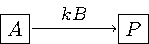
\includegraphics{series_files/figure-latex/mass-action-1} 

}

\caption{Schematic diagram of a substrate-enzyme reaction.}\label{fig:mass-action}
\end{figure}

One key quantity is the rate of formation for the product \(P\), which we express by Equation \eqref{eq:mass-action}:

\begin{equation}
\frac{dP}{dt}= kAB, \label{eq:mass-action}
\end{equation}

where \(k\) is the proportionality constant or the rate constant associated with the reaction. Notice how we express the interaction between \(A\) and \(B\) as a product - if either the substrate \(A\) or enzyme \(B\) is not present (i.e.~\(A\) or \(B\) equal 0), then product \(P\) is not formed. Equation \eqref{eq:mass-action} is an example of the law of mass action.\index{mass action}

Modeling interactions (whether between susceptible and infected individuals, enzymes and substrates, or predators and prey) with the law of mass action is always a good first assumption to understand the system, which can be subsequently refined. For example, if we consider that the substrate might decay, we can revise Figure \ref{fig:mass-action} to Figure \ref{fig:mass-action-revised}:

\begin{figure}

{\centering 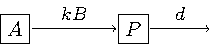
\includegraphics{series_files/figure-latex/mass-action-revised-1} 

}

\caption{Revised schematic diagram of substrate-enzyme reaction with deacy of the product $P$.}\label{fig:mass-action-revised}
\end{figure}

In this instance the rate of change of \(P\) would then include a term \(dP\) (Equation \eqref{eq:mass-action-decay}:

\begin{equation}
\frac{dP}{dt}= kAB - dP, \label{eq:mass-action-decay}
\end{equation}

\hypertarget{coupled-differential-equations-lynx-and-hares}{%
\section{Coupled differential equations: lynx and hares}\label{coupled-differential-equations-lynx-and-hares}}

Another example is a \emph{system of differential equations}.\index{differential equation!system of equations} The context is between the snowshoe hare and the Canadian lynx, shown in Figure \ref{fig:lynx-hare}. Figure \ref{fig:lynx-hare-time} also displays a timeseries of the two populations overlaid. Notice how in Figure \ref{fig:lynx-hare-time} both populations show regular periodic fluctuations. One plausible reason is that the lynx prey on the snowshoe hares, which causes the population to initially decline. Once the snowshoe hare population declines, then there is less food for the lynx to survive, so their population declines. The decline in the lynx population causes the hare population to increase, and the cycle repeats.\footnote{There is a lot more nuance for reasons behind periodic fluctuations in these two populations, which includes more complicated food web interactions and climate variation. \protect\hyperlink{ref-maclulich_fluctuations_1937}{MacLulich} (\protect\hyperlink{ref-maclulich_fluctuations_1937}{1937}), \protect\hyperlink{ref-stenseth_population_1997}{Stenseth et al.} (\protect\hyperlink{ref-stenseth_population_1997}{1997}), and \protect\hyperlink{ref-king_geometry_2001}{King and Schaffer} (\protect\hyperlink{ref-king_geometry_2001}{2001}) are good places to dig into the complexity of this fascinating biological system. ~ Image sources for Figure \ref{lynx-hare}: \protect\hyperlink{ref-usa_canada_2012}{Kilby} (\protect\hyperlink{ref-usa_canada_2012}{2012}) and \protect\hyperlink{ref-preserve_snowshoe_2011}{Frank, Jacob W.} (\protect\hyperlink{ref-preserve_snowshoe_2011}{2021}). Image source for Figure \ref{fig:lynx-hare-time}: \protect\hyperlink{ref-openstax_notitle_2016}{OpenStax} (\protect\hyperlink{ref-openstax_notitle_2016}{2016})}

\begin{figure}

{\centering 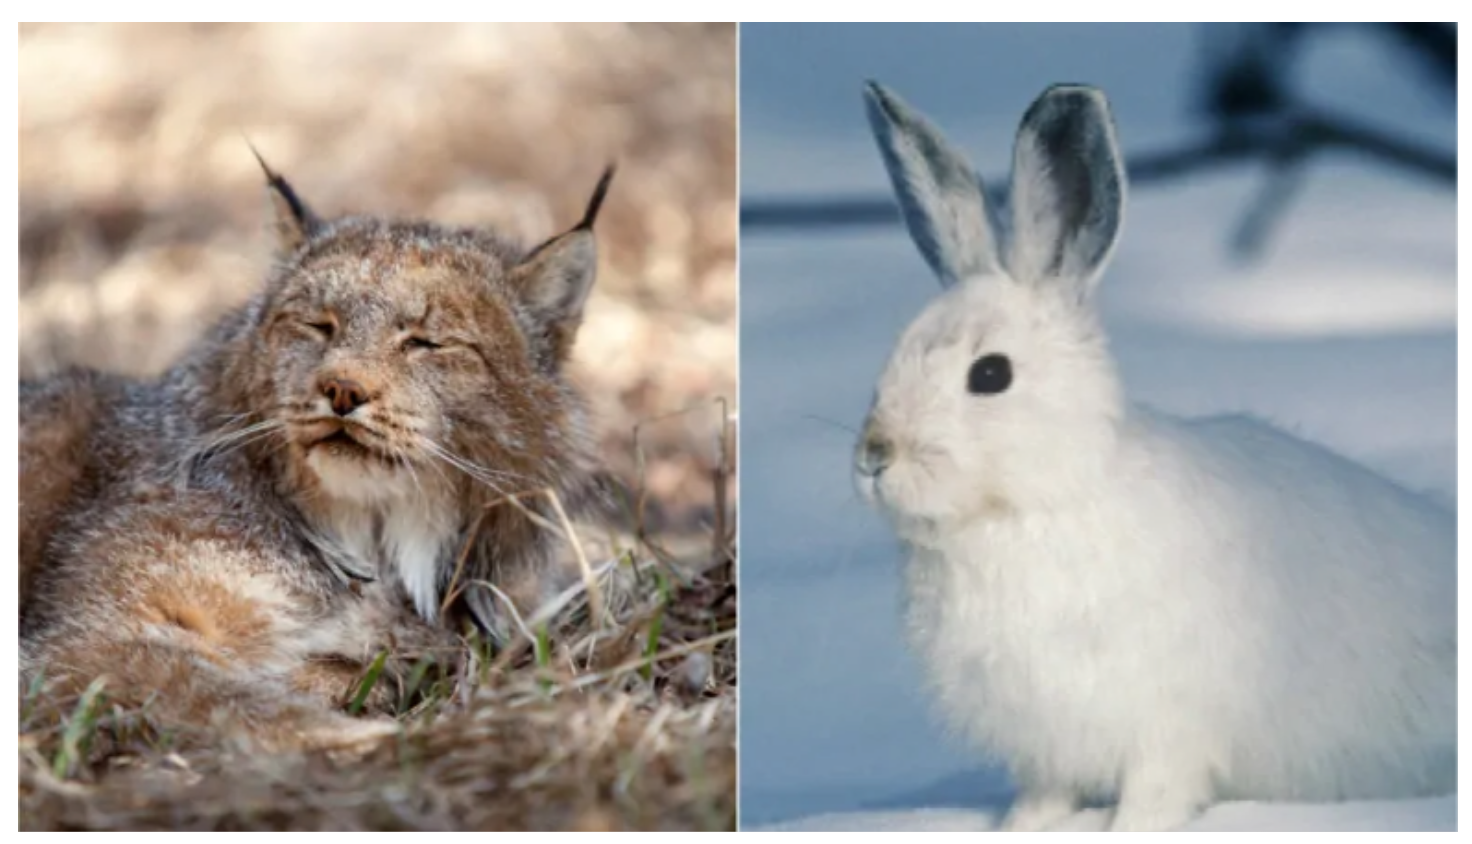
\includegraphics[width=0.7\linewidth]{figures/03-systems/lynx-hare} 

}

\caption{Examples of lynx and hare - aren't they beautiful?}\label{fig:lynx-hare}
\end{figure}

\begin{figure}

{\centering 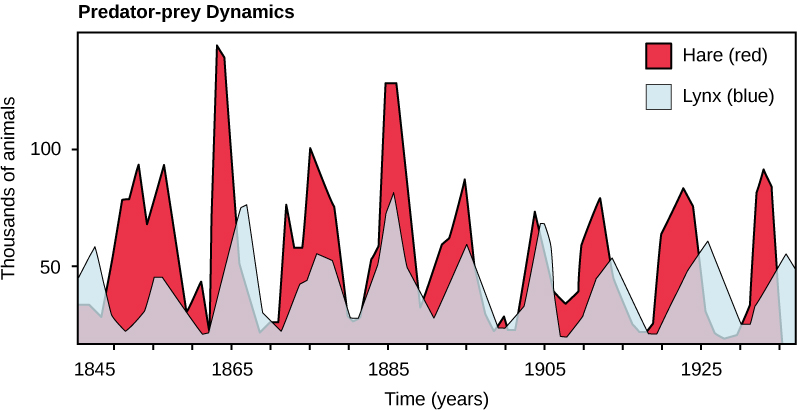
\includegraphics[width=0.7\linewidth]{figures/03-systems/Figure_45_06_01} 

}

\caption{Timeseries of the combined lynx and hare populations. Notice how the populations are coupled with each other.}\label{fig:lynx-hare-time}
\end{figure}

In summary it is safe to say that the two populations are \emph{coupled} to one another, yielding a coupled system of equations.\index{differential equation!coupled system} But in order to understand how they are coupled together, first let's consider the two populations \emph{separately}.

To develop the mathematical model we will make some simplifying assumptions. The hares grow much more quickly than then lynx - in fact some hares have been known to reproduce several times a year. A reasonable assumption for large hare populations is that rate of change of the hares is proportional to the hare population. Based on this assumption Equation \eqref{eq:hareOnly} describes the rate of change of the hare population, with \(H\) is the population of the hares:

\begin{equation}
\frac{dH}{dt} = r H \label{eq:hareOnly}
\end{equation}

Since the growth rate \(r\) is positive, so then the rate of change (\(H'\)) will be positive as well, and \(H\) will be increasing. A representative value for \(r\) is 0.5 year\(^{-1}\) \protect\hyperlink{ref-brady_circle_2021}{Brady and Butler} (\protect\hyperlink{ref-brady_circle_2021}{2021}). You may be thinking that the units on \(r\) seem odd - (year\(^{-1}\)), but that unit on \(r\) makes the term \(rH\) dimensionally consistent to be a rate of change.

Let's consider the lynx now. A approach is to assume their population declines exponentially, or changes at the rate proportional to the current population. Let's consider \(L\) to be the lynx population, with the following differential equation (Equation \eqref{eq:lynxOnly}):

\begin{equation}
\frac{dL}{dt} = -dL \label{eq:lynxOnly}
\end{equation}

We assume the death rate \(d\) in Equation \eqref{eq:lynxOnly} is positive, leading to a negative rate of change for the Lynx population (and a decreasing value for \(L\)). A typical values of \(d\) is 0.9 yr\(^{-1}\) \protect\hyperlink{ref-brady_circle_2021}{Brady and Butler} (\protect\hyperlink{ref-brady_circle_2021}{2021}).

The next part to consider is how the lynx and hare interact. Since the hares are prey for the lynx, when the lynx hunt, the hare population decreases. We can represent the process of hunting with the following adjustment to our hare equation:

\begin{equation}
\frac{dH}{dt} = r H - b HL
\end{equation}

So the parameter \(b\) represents the hunting rate. Notice how we have the term \(HL\) for this interaction. This term injects a sense of realism: if the lynx are not present (\(L=0\)), then the hare population can't decrease due to hunting. We say that the \emph{interaction} between the hares and the lynx with multiplication. A typical value for \(b\) is .024 lynx\(^{-1}\) year\(^{-1}\). It is okay if that unit seems a little odd to you - it should be! As before, if we multiply out the units on \(bHL\) we would get units of hares per year.

How does hunting affect the lynx population? One possibility is that it increases the lynx population:

\begin{equation}
\frac{dL}{dt} =bHL -dL
\end{equation}

Notice the symmetry between the rate of change for the hares and the lynx equations. In many cases this makes sense - if you subtract a rate from one population, then that rate should be added to the receiving population. You could also argue that there is some efficiency loss in converting the hares to lynx - not all of the hare is converted into lynx biomass. In this situation we sometimes like to adjust the hunting term for the lynx equation with another parameter \(e\), representing the efficiency that hares are converted into lynx:

\begin{equation}
\frac{dL}{dt} =e \, bHL -dL
\end{equation}

(sometimes people just make a new parameter \(c=e \, b\), but for now we will just leave it as is and set \(e=0.2\)). Equation \eqref{eq:lynx-hare-combined} shows the coupled system of differential equations:

\begin{equation}
\begin{split}
\frac{dH}{dt} &= r H - b HL \\
\frac{dL}{dt} &=e\,bHL -dL
\end{split}
\label{eq:lynx-hare-combined}
\end{equation}

The schematic diagram representing these interactions is the following is shown in Figure \ref{fig:lynxhare-schematic}:

\begin{figure}

{\centering 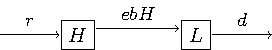
\includegraphics{series_files/figure-latex/lynxhare-schematic-1} 

}

\caption{Schematic diagram Lynx-Hare system.}\label{fig:lynxhare-schematic}
\end{figure}

Equation \eqref{eq:lynx-hare-combined} is a classical model in mathematical biology and differential equations - it is called the \emph{predator prey} model, also known as the \emph{Lotka-Volterra model} \protect\hyperlink{ref-volterra_fluctuations_1926}{Volterra} (\protect\hyperlink{ref-volterra_fluctuations_1926}{1926}).\index{model!predator-prey}\index{model!Lotka-Volterra}

\hypertarget{functional-responses}{%
\section{Functional responses}\label{functional-responses}}

In several examples we have seen a rate of change proportional to the current population, as in the rate of growth of the hare population is \(rH\). This is one example of what we would call a \href{https://en.wikipedia.org/wiki/Functional_response}{functional response}.\index{functional response} Another type of functional response assumes that the rate reaches a limiting value proportional to the population size, so \(\displaystyle \frac{dH}{dt} = \frac{rH}{1+arH}\). This is an example of a \textbf{type II functional response}.\index{functional response!type II} Finally, the type II response has also been generalized (a \textbf{type III functional response}) \(\displaystyle \frac{dH}{dt} = \frac{rH^{2}}{1+arH^{2}}\).\index{functional response!type III} Figure \ref{fig:function-response} shows all three functional responses together:

\begin{figure}
\centering
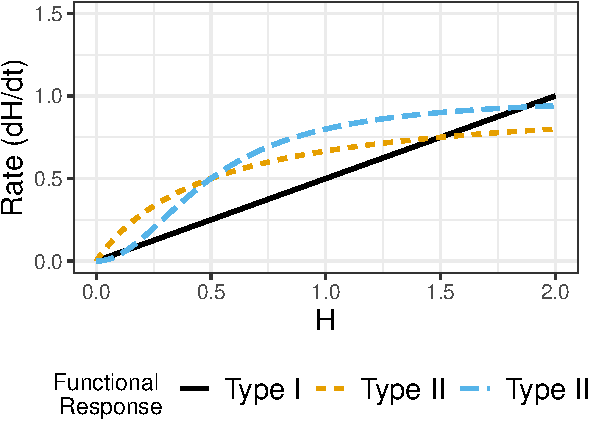
\includegraphics{series_files/figure-latex/function-response-1.pdf}
\caption{\label{fig:function-response}Comparison between examples of Type I - Type III functional responses. For a Type I functional response the Rate grows proportional to population size \emph{H}, whereas for Types II and III the rate reaches a saturating value.}
\end{figure}

Notice the limiting behavior in the Type II and Type III functional responses. These responses are commonly used in ecology and predator-prey dynamics and in problems of how animals search for food.

\hypertarget{exercises}{%
\section{Exercises}\label{exercises}}

\begin{exercise}
\protect\hypertarget{exr:unnamed-chunk-3}{}{\label{exr:unnamed-chunk-3} }Consider the following type of functional responses:

\begin{equation}
\begin{split}
\mbox{ Type I: } \frac{dP}{dt} &= 0.1 P \\
\mbox{ Type II: } \frac{dP}{dt} &= \frac{0.1P}{1+.03P} \\
\mbox{ Type III: } \frac{dP}{dt} &= \frac{0.1P^{2}}{1+.05P^{2}}
\end{split}
\end{equation}

For each of the functional responses evaluate \(\displaystyle \lim_{P \rightarrow \infty} \frac{dP}{dt}\). Since these functional responses represent a rate of change of a population, what are some examples (hypothetical or actual) would each of these responses be appropriate?
\end{exercise}

\begin{exercise}
\protect\hypertarget{exr:unnamed-chunk-4}{}{\label{exr:unnamed-chunk-4} }A population grows according to the equation:

\begin{equation}
\frac{dP}{dt} = \frac{0.1P}{1+.05P} -P = f(P) - g(P)
\end{equation}

\begin{enumerate}
\def\labelenumi{\alph{enumi}.}
\tightlist
\item
  On the same axis, plot the equations \(f(P)\) and \(g(P)\). What are the two positive values of \(P\) where \(f(P)\) and \(g(P)\) intersect?
\item
  Next algebraically determine the two steady state values of \(P\), that is solve \(\displaystyle \frac{dP}{dt}=0\) for \(P\). (\emph{Hint:} factor a \(P\) out of the expression \(\displaystyle f(P)-g(P)\).)
\item
  Does your algebraic solution match your graphical solutions?
\end{enumerate}
\end{exercise}

\begin{exercise}
\protect\hypertarget{exr:unnamed-chunk-5}{}{\label{exr:unnamed-chunk-5} }A population grows according to the equation:

\begin{equation}
\frac{dP}{dt} = 2P - \frac{4P^{2}}{1+P^{2}} = r(P)-d(P)
\end{equation}

\begin{enumerate}
\def\labelenumi{\alph{enumi}.}
\tightlist
\item
  On the same axis, plot the equations \(r(P)\) and \(d(P)\). What are the two positive values of \(P\) where \(r(P)\) and \(d(P)\) intersect?
\item
  Next algebraically determine the two steady state values of \(P\), that is solve \(\displaystyle \frac{dP}{dt}=0\) for \(P\). (\emph{Hint:} factor a \(P\) out of the expression \(r(P)-d(P)\).)
\item
  Does your algebraic solution match your graphical solutions?
\end{enumerate}
\end{exercise}

\begin{exercise}
\protect\hypertarget{exr:unnamed-chunk-6}{}{\label{exr:unnamed-chunk-6} }A population grows according to the equation:

\begin{equation}
\frac{dP}{dt} = \frac{aP}{1+abP} - dP,
\end{equation}

where \(a\), \(b\) and \(d\) are all positive parameters. Determine the two steady state values of \(P\), that is solve \(\displaystyle \frac{dP}{dt}=0\) for \(P\).
\end{exercise}

\begin{exercise}
\protect\hypertarget{exr:unnamed-chunk-7}{}{\label{exr:unnamed-chunk-7} }A chemical reaction takes two chemicals \(X\) and \(Y\) to form a substrate \(Z\) through the law of mass action. However the substrate can also disassociate. The reaction schematic is the following:

\begin{equation}
X + Y \rightleftharpoons Z,
\end{equation}

where you may define a the proportionality constant \(k_+\) is associated with the formation of the substrate \(Z\) and \(k_-\) the disassociation (\(Z\) decays back to \(X\) and \(Y\)).

~

Write down a differential equation that represents the rate of reaction \(\displaystyle \frac{dZ}{dt}\).
\end{exercise}

\begin{exercise}
\protect\hypertarget{exr:unnamed-chunk-8}{}{\label{exr:unnamed-chunk-8} }(Inspired from \protect\hyperlink{ref-thornley_plant_1990}{Thornley and Johnson} (\protect\hyperlink{ref-thornley_plant_1990}{1990}) and \protect\hyperlink{ref-logan_mathematical_2009}{Logan and Wolesensky} (\protect\hyperlink{ref-logan_mathematical_2009}{2009})) For each of the following exercises consider the following contextual situations modeling rates of change. For each problem you will need to:

\begin{itemize}
\tightlist
\item
  Name and describe all variables and parameters.
\item
  Determine a differential equation representing the context.
\item
  Write a brief one-two sentence explanation of why your differential equation models the situation at hand.
\item
  Hand sketch a rough graph of what you think the solution as a function of time, consistent with the context given.
\end{itemize}

\begin{enumerate}
\def\labelenumi{\alph{enumi}.}
\tightlist
\item
  The rate of change of an animal's body temperature is proportional to the difference in temperature between the environment.
\item
  A plant grows propritional to its current length \(L\). Assume this proportionality constant is \(\mu\), whose rate also decreases proportional to its current value. You will need to write down a system of two equation with variables \(L\) and \(\mu\).
\item
  A patient undergoing chemotherapy receives an injection at rate \(I\). This injection decreases the rate that a tumor accumulates mass. Independent of the injection, the tumor accumulates mass at a rate proportional to the mass of the tumor.
\item
  A cell with radius \(r\) assimilates nutrients at a rate proportional to its surface area, but uses nutrients proportional to its volume. Determine an equation that represents the rate of change of the radius.
\item
  A patient undergoing chemotherapy receives an injection at rate \(I\). This injection decreases the rate that a tumor accumulates mass. Independent of the injection, the tumor accumulates mass at a rate proportional to the mass of the tumor.
\item
  The rate that a cancer cell divides (increases in amount) is proportional to the amount of healthy cells in its surrounding environment. You may assume that a healthy cell has a mortality \(\delta_{H}\) and a cancer cell has mortality \(\delta_{C}\). Be sure to write down a system of differential equations for the population of cancer cells \(C\) and healthy cells \(H\).
\item
  The rate that a virus is spread to the population is proportional to the probability that a person is sick (out of \(N\) total sick and healthy individuals).
\end{enumerate}
\end{exercise}

\begin{figure}
\centering
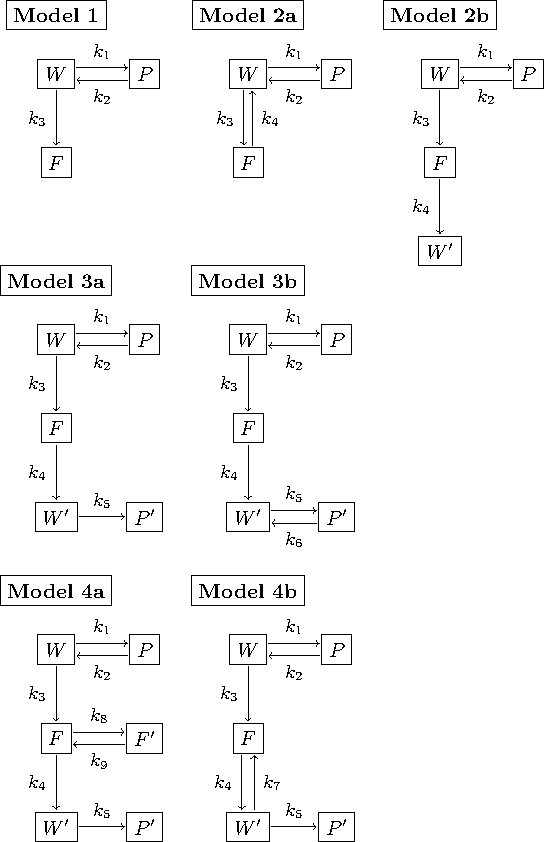
\includegraphics{series_files/figure-latex/pesticide-ch3-1.pdf}
\caption{\label{fig:pesticide-ch3}Modeled reaction schemes representing the potential effect of a pesticide on water quality.}
\end{figure}

\begin{exercise}
\protect\hypertarget{exr:unnamed-chunk-9}{}{\label{exr:unnamed-chunk-9} }(Inspired by \protect\hyperlink{ref-burnham_model_2002}{Burnham and Anderson} (\protect\hyperlink{ref-burnham_model_2002}{2002})) You are tasked with the job of investigating the effect of a pesticide on water quality, in terms of its effects on the health of the plants and fish in the ecosystem. Different models can be created that investigate the effect of the pesticide. Different types of reaction schemes for this system are shown in Figure \ref{fig:pesticide-ch3}, where \(F\) represents the amount of pesticide in the fish, \(W\) the amount of pesticide in the water, and \(S\) the amount of pesticide in the soil. The prime (e.g.~\(F'\), \(W'\), and \(S'\) represent other bound forms of the respective state). In all seven different models can be derived. For each of the model schematics, apply the Law of Mass Action to write down a system of differential equations.
\end{exercise}

\hypertarget{references}{%
\chapter*{References}\label{references}}


\hypertarget{refs}{}
\begin{CSLReferences}{1}{0}
\leavevmode\hypertarget{ref-brady_circle_2021}{}%
Brady, R, and J Butler. 2021. {``The {Circle} of {Life}: {The Mathematics} of {Predator-Prey Relationships}.''} \emph{Frontiers for Young Minds} 9 (651131). \url{https://kids.frontiersin.org/articles/10.3389/frym.2021.651131}.

\leavevmode\hypertarget{ref-R-formula.tools}{}%
Brown, Christopher. 2018. \emph{Formula.tools: Programmatic Utilities for Manipulating Formulas, Expressions, Calls, Assignments and Other r Objects}. \url{https://github.com/decisionpatterns/formula.tools}.

\leavevmode\hypertarget{ref-burnham_model_2002}{}%
Burnham, Kenneth P., and David R. Anderson. 2002. \emph{Model {Selection} and {Multimodel Inference}}. {New York, NY}: {Springer New York}.

\leavevmode\hypertarget{ref-preserve_snowshoe_2011}{}%
Frank, Jacob W. 2021. {``Snowshoe {Hare}.''} \url{https://commons.wikimedia.org/wiki/File:Snowshoe/_Hare/_(6187109754).jpg}.

\leavevmode\hypertarget{ref-R-expm}{}%
Goulet, Vincent, Christophe Dutang, Martin Maechler, David Firth, Marina Shapira, and Michael Stadelmann. 2021. \emph{Expm: Matrix Exponential, Log, Etc}. \url{http://R-Forge.R-project.org/projects/expm/}.

\leavevmode\hypertarget{ref-usa_canada_2012}{}%
Kilby, Eric. 2012. {``Canada {Lynx}.''} \url{https://commons.wikimedia.org/wiki/File:Canada/_Lynx/_(8154273321).jpg}.

\leavevmode\hypertarget{ref-king_geometry_2001}{}%
King, Aaron A., and William M. Schaffer. 2001. {``The {Geometry} of a {Population Cycle}: {A Mechanistic Model} of {Snowshoe Hare Demography}.''} \emph{Ecology} 82 (3): 814--30. \url{https://doi.org/10.2307/2680200}.

\leavevmode\hypertarget{ref-logan_mathematical_2009}{}%
Logan, J. David, and William Wolesensky. 2009. \emph{Mathematical {Methods} in {Biology}}. 1st ed. {Hoboken, N.J}: {W}iley.

\leavevmode\hypertarget{ref-lotka_analytical_1920}{}%
Lotka, Alfred J. 1920. {``Analytical {Note} on {Certain Rhythmic Relations} in {Organic Systems}.''} \emph{Proceedings of the National Academy of Science} 6 (7): 410--15.

\leavevmode\hypertarget{ref-lotka_elements_1926}{}%
---------. 1926. {``Elements of {Physical Biology}.''} \emph{Science Progress in the Twentieth Century (1919-1933)} 21 (82): 341--43.

\leavevmode\hypertarget{ref-maclulich_fluctuations_1937}{}%
MacLulich, D. A. 1937. \emph{Fluctuations in the {Numbers} of the {Varying Hare} ({Lepus Americanus})}. Toronto, Canada: {University of Toronto Press}. \url{https://doi.org/10.3138/9781487583064}.

\leavevmode\hypertarget{ref-mahaffy_lotka-volterra_2010}{}%
Mahaffy, Joseph. 2010. {``Lotka-{Volterra Models}.''} \url{https://jmahaffy.sdsu.edu/courses/f09/math636/lectures/lotka/qualde2.html}.

\leavevmode\hypertarget{ref-openstax_notitle_2016}{}%
OpenStax, C. N. X. 2016. \url{https://commons.wikimedia.org/wiki/File:Figure/_45/_06/_01.jpg}.

\leavevmode\hypertarget{ref-R-base}{}%
R Core Team. 2021. \emph{R: A Language and Environment for Statistical Computing}. Vienna, Austria: R Foundation for Statistical Computing. \url{https://www.R-project.org/}.

\leavevmode\hypertarget{ref-rstudio_team_rstudio_2020}{}%
RStudio Team. 2020. \emph{{RStudio}: {Integrated} Development Environment for r}. Manual. {Boston, MA}: {RStudio, PBC}. \url{http://www.rstudio.com/}.

\leavevmode\hypertarget{ref-R-GGally}{}%
Schloerke, Barret, Di Cook, Joseph Larmarange, Francois Briatte, Moritz Marbach, Edwin Thoen, Amos Elberg, and Jason Crowley. 2021. \emph{GGally: Extension to Ggplot2}. \url{https://CRAN.R-project.org/package=GGally}.

\leavevmode\hypertarget{ref-stenseth_population_1997}{}%
Stenseth, Nils Chr, Wilhelm Falck, Ottar N. Bjørnstad, and Charles J. Krebs. 1997. {``Population Regulation in Snowshoe Hare and {Canadian} Lynx: {Asymmetric} Food Web Configurations Between Hare and Lynx.''} \emph{Proceedings of the National Academy of Sciences} 94 (10): 5147--52. \url{https://doi.org/10.1073/pnas.94.10.5147}.

\leavevmode\hypertarget{ref-thornley_plant_1990}{}%
Thornley, John H M, and Ian R Johnson. 1990. \emph{Plant and {Crop Modelling}: {A Mathematical Approach} to {Plant} and {Crop Physiology}}. Caldwell, New Jersey: {Blackburn Press}.

\leavevmode\hypertarget{ref-volterra_fluctuations_1926}{}%
Volterra, Vito. 1926. {``Fluctuations in the {Abundance} of a {Species} Considered {Mathematically}.''} \emph{Nature} 118 (2972): 558--60. \url{https://doi.org/10.1038/118558a0}.

\leavevmode\hypertarget{ref-tidyverse2019}{}%
Wickham, Hadley, Mara Averick, Jennifer Bryan, Winston Chang, Lucy D'Agostino McGowan, Romain François, Garrett Grolemund, et al. 2019. {``Welcome to the {tidyverse}.''} \emph{Journal of Open Source Software} 4 (43): 1686. \url{https://doi.org/10.21105/joss.01686}.

\end{CSLReferences}

\backmatter
\printindex

\end{document}
